\chapter{Wiederholung}
\renewcommand{\chaptertitle}{Wiederholung}

\lehead[]{\normalfont\sffamily\hspace*{-2.00cm}\textcolor{white}{\colorbox{lightblue}{\parbox[c][0.70cm][b]{1.60cm}{
\makebox[1.60cm][r]{\thechapter}\\ \makebox[1.60cm][r]{ÜBUNG}}}}\hspace{0.17cm}\textcolor{lightblue}{\chaptertitle}}
\rohead[]{\textcolor{lightblue}{\chaptertitle}\normalfont\sffamily\hspace*{0.17cm}\textcolor{white}{\colorbox{lightblue}{\parbox[c][0.70cm][b]{1.60cm}{\thechapter\\
ÜBUNG}}}\hspace{-2.00cm}}
%\chead[]{}
\rehead[]{\textcolor{lightblue}{AvHG, Inf, My}}
\lohead[]{\textcolor{lightblue}{AvHG, Inf, My}}

\lstset{style=myJava}

\section{Programmierung}

\subsection{Aufgabe 1: Kette}

\begin{compactenum}[a)]
\item Erzeuge ein Anwendungsfenster mit einem schwarzen Hintergrund. Das
Anwendungsfenster soll eine Breite und Höhe von je 500 Pixel besitzen.

\item Programmiere eine Klasse \myClass{Kreis}. Ein Kreis besitzt private
Attribute für Farbe, x-Position und y-Position. Alle drei genannten Eigenschaften werden im
Konstruktor als Parameter übergeben. Die Breite des Kreises wird mit einer
Konstanten auf 40 Pixel festgesetzt. Es gibt eine Methode \verb|zeichnen()|, die
einen ausgefüllten Kreis an der (x,y)-Position mit der eingestellten Farbe
zeichnet. Überlege dir selber, welche Parameter und welcher Rückgabewert für
die Methode \verb|zeichnen()| sinnvoll sind.

Zur Lösung der weiteren Aufgaben darf die Klasse \myClass{Kreis} zusätzliche
Attribute erhalten, die jedoch vor einem Zugriff von außen geschützt werden müssen.

\item Programmiere eine Klasse \myClass{Kette}. Eine Kette besteht aus sechs
Objekten der Klasse \myClass{Kreis}, die wie folgt angeordnet werden sollen:

\begin{center}
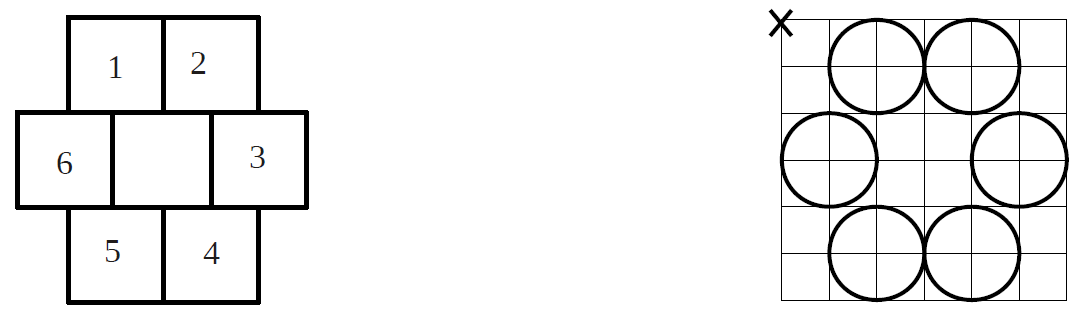
\includegraphics[width=0.7\textwidth]{./inf/SEKII/17_Java_Wiederholung/Aufgabe1.png}
\end{center}

Die rechte Abbildung zeigt wie die Kette aussehen soll. Die linke
Abbildung zeigt die Quadrate, durch die die Kreise beschrieben werden. Die
Ziffern innerhalb der Quadrate geben die Reihenfolge an, in der die
Kreis-Objekte erzeugt werden sollen. Bitte halte dich an diese Reihenfolge,
weil sie für die weiteren Aufgaben von Bedeutung ist. Ein Karo-Kästchen
entspricht einer Breite von 20 Pixel. Das Kreuz markiert die linke obere Ecke
der Kette und soll nicht mit gezeichnet werden.

Im Konstruktor der Kette werden die Farbe und die linke obere Ecke der Kette
übergeben (x- und y- Position). Alle Kreis-Objekte erhalten die in der Kette
übergebene Farbe. Es gibt eine Methode \verb|zeichnen()|, die die Kette an der
angegebenen Position zeichnet.

Erzeuge im Anwendungsfenster drei Objekte von der Kette:
\begin{compactitem}
\item Das erste Objekt erhält die Farbe rot und die linke obere Ecke (180 | 100).
\item Das zweite Objekt erhält die Farbe blau und die linke obere Ecke (50 | 250).
\item Das dritte Objekt erhält die Farbe grün und die linke obere Ecke (300 | 250).
\end{compactitem}

\item Füge in das Anwendungsfenster ein Objekt der Klasse \myClass{Timer} ein
und sorge dafür, dass das Fenster alle 500 Millisekunden neu gezeichnet wird.

Erweitere anschließend die Klasse \myClass{Kreis}. Bei jedem dritten Aufruf der
Methode \verb|zeichnen()| wird das \myClass{Kreis}-Objekt nicht in seiner
eingestellten Farbe sondern mit der Farbe orange gezeichnet. Dadurch erhält die
gesamte Kette bei jedem dritten Aufruf von \verb|zeichnen()| die Farbe orange.

\item Erweitere die Klasse \myClass{Kreis} noch einmal. Die Kreis-Objekte sollen
jetzt nicht mehr alle zur gleichen Zeit die Farbe orange anzeigen. Die Kreise
werden beim Erzeugen der Objekte zyklisch durchgezählt: 1, 2, 3, 1, 2, 3, 1, 2,
3, \ldots .

Jedes erste \myClass{Kreis}-Objekt hat den Rhythmus: farbe, farbe, orange,
farbe, farbe, orange, \ldots

Jedes zweite \myClass{Kreis}-Objekt hat den Rhythmus: farbe, orange, farbe,
farbe, orange, farbe \ldots

Jedes dritte \myClass{Kreis}-Objekt hat den Rhythmus: orange, farbe, farbe,
orange, farbe, farbe, \ldots

Dadurch gibt es in jeder Kette immer zwei orange Kugeln zur Zeit. Die
orange Farbe wandert von einer Kugel zur anderen.

\item Füge in die Klasse \myClass{Kette} ein Objekt der Klasse \myClass{Random}
ein. Das \myClass{Random}-Objekt darf nur in der gesamten Klasse \myClass{Kette}
nur einmal vorkommen.

Erweitere die Klasse \myClass{Kette} nun folgendermaßen: Jede Kette wird
abwechselnd eine zufällige Zeitspanne lang ausgeschaltet (das heißt sie ist
nicht sichtbar) und danach wieder eine zufällige Zeitspanne lang angeschaltet.
Die Zufallswerte werden für jeden „An“ bzw. „Aus“-Zyklus neu erzeugt und sollen
zwischen 5 und 15 liegen. Die Zufallszahl 6 bedeutet beispielsweise, dass die
Kette über 6 Aufrufe von \verb|zeichnen()| nicht zu sehen ist.

\end{compactenum}


\subsection{Aufgabe 2: Kreisende Bälle}

\begin{compactenum}[a)]

\item Erzeuge ein Anwendungsfenster mit einem schwarzen Hintergrund und weißer
Vordergrundfarbe. Das Anwendungsfenster soll eine Breite und Höhe von je 500
Pixel besitzen.

\item Programmiere in einer zweiten Datei eine Klasse \myClass{Ball}. Alle
Attribute der Klasse \myClass{Ball} sollen vor dem Zugriff von außen (d.h. vom
Anwendungsfenster aus) geschützt sein. Alle Methoden sind öffentlich und dürfen
vom Anwendungsfenster  aus benutzt werden.

\item Ein Ball besitzt zu Anfang die Attribute x-Position, y-Position, Breite
und Farbe. Weitere Attribute dürfen später nach Bedarf hinzugefügt werden. Die
x-Position wird automatisch auf den Wert 25 festgelegt, die y-Position auf den
Wert 250 und die Breite auf den Wert 50. Nur die Farbe kann vom
Anwendungsfenster aus eingestellt werden und wird im Konstruktor als Parameter
übergeben.

Schreibe eine Methode \verb|zeichnen()|, die den Ball an seiner aktuellen
Position und in der für ihn gewählten Farbe als ausgefüllten Kreis zeichnet.
Entscheide selbst welche Parameter und welchen Rückgabewert die Methode
\verb|zeichnen()| benötigt.

\item Erzeuge im Anwendungsfenster ein Objekt der Klasse Ball, das eine rote
Farbe besitzt.

\item Füge im Anwendungsfenster ein Objekt der Klasse \myClass{Timer} ein, und
stelle den Timer so ein, dass die \verb|myPaint()|-Methode alle 10 Millisekunden
aufgerufen wird.

\item Erweitere in der Klasse \myClass{Ball} die Methode \verb|zeichnen()|, so
dass in der Methode die x-Position des Balls bei jedem Aufruf um zwei Pixel
verschoben wird. Der Ball soll immer abwechselnd zunächst nach rechts rollen
bis zur x-Position 425 und anschließend wieder zurück nach links bis zur
x-Position 25.

\item Erweitere die Klasse Ball so, dass jedes weitere Ball-Objekt automatisch
in seiner anfänglichen x- Position um 50 Pixel nach rechts verschoben wird. Das
erste Ball-Objekt besitzt bei Erzeugung die x- Position 25, das zweite
Ball-Objekt die x-Position 75, das dritte Ball-Objekt die x-Position 125, usw.

Erzeuge im Anwendungsfenster acht verschiedene Ball-Objekte, die
unterschiedliche Farben besitzen sollen. Die Farben darfst du frei wählen. Wenn
du alles richtig gemacht hast, bilden die Ball-Objekte eine Art „Schlange“.

\item Die Klasse \myClass{Ball} soll so erweitert werden, dass sich der Ball im
Uhrzeigersinn im Kreis bewegt. Wenn der Ball sich nach rechts bewegt, wird die
y-Koordinate in Abhängigkeit von der x-Koordinate folgendermaßen berechnet:

\begin{lstlisting}
y = 250 - (int) Math.sqrt(40000-(x-225)*(x-225));
\end{lstlisting}

Dadurch bewegt sich der Ball im Halbkreis nach oben. Wenn sich der Ball nach
links bewegt, wird die y- Koordinate mit der Formel

\begin{lstlisting}
y = 250 + (int) Math.sqrt(40000-(x-225)*(x-225));
\end{lstlisting}

berechnet. Dadurch bewegt sich der Ball im Halbkreis nach unten. Beachte, dass
der Ball bei dieser Technik an den Seiten links und rechts wesentlich schneller
rollt als in der Mitte. Das ist kein Programmierfehler.

Vorgabe: Berechne die y-Koordinate für den Ball mit Hilfe einer Methode, die
die x-Koordinate als Parameter erhält und die y-Koordinate als Rückgabewert
zurück gibt. Schreibe entweder für jede der beiden Formeln eine Methode oder
programmiere eine einzige Methode, die die aktuelle Richtung des Balls
berücksichtigt.

\item Erweitere die Klasse \myClass{Ball} so, dass ein Ball zyklisch immer
zweimal im Kreis rollt und dann einmal wie in Teilaufgabe e) mit fester
y-Koordinate nach rechts und wieder zurück nach links rollt. Das heißt, die
Berechnung der y-Koordinate mit den Kreis-Formeln entfällt bei jedem dritten
Durchgang.

\end{compactenum}